%------------------------------------------------
\section{Desenvolvimento e resultados}
%------------------------------------------------

%%%%%%%%%%%%%%%%%%%%%%%%%%%%%%%%%%%%%%%%%%%%%%%%%%%%%%%%%%%
%%%%%%%%%%%%%%%%%%%%%%%%%%%%%%%%%%%%%%%%%%%%%%%%%%%%%%%%%%%

\subsection{O Projeto}

\begin{frame}
\frametitle{O Projeto}
\begin{enumerate}
\item Estudo da tecnologia;
\pause \item Comparativo entre os módulos;
\pause \item Implementação no microcontrolador.
\end{enumerate}
\end{frame}

\subsection{Estudo da tecnologia}

\begin{frame}
\frametitle{Estudo da tecnologia}
\begin{itemize}
\item Estudo do NMEA;
\pause
\item Estudo dos módulos de GPS da u-blocks:
	\begin{itemize}
	\item NEO-6M;
	\item LEA-6H;
	\end{itemize}
\pause
\item IDE Coocox e bibliotecas CMSIS;
\end{itemize}
\end{frame}

\subsection{Comparativo entre os módulos}

\begin{frame}
\frametitle{Comparativo entre os módulos}
\begin{columns}

	\column{0.4\linewidth}
	\begin{itemize}
	\item Comparação feita com o Arduino;
	\item Informações salvas em um cartão SD;
	\item Testes definitivos feitos na pista de atletismo da UTFPR;
	\item Informações graficadas no \textit{software} Google Earth;
	\item Desenvolvimento de uma \textit{shield} para o Arduino Mega;
	\end{itemize}

	\column{0.7\linewidth}
	\begin{figure}[]
	 \centering
	 \captionsetup{width=0.9\textwidth,font=footnotesize,textfont=bf}
	 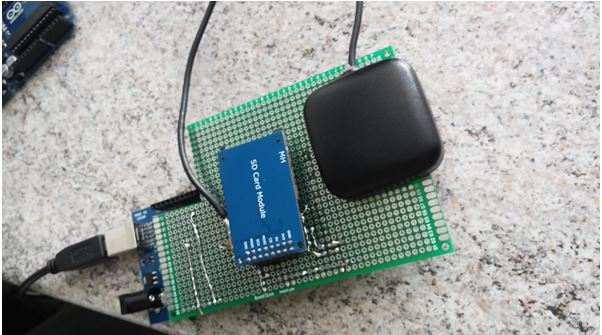
\includegraphics[width=0.9\textwidth,keepaspectratio]{Figuras/shield.jpg}
	 \caption{Shield para o Arduino}
	\end{figure}
	
\end{columns}
\end{frame}




\begin{frame}
\frametitle{Comparativo entre os módulos}

	\begin{figure}[]
	 \centering
	 \captionsetup{width=0.9\textwidth,font=footnotesize,textfont=bf}
	 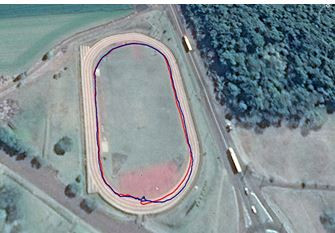
\includegraphics[width=0.9\textwidth,keepaspectratio]{Figuras/teste.jpg}
	 \caption{Comparativo entre os dois módulos (Vermelho: LEA-6H; Azul: NEO-6M)}
	\end{figure}
\end{frame}



\begin{frame}
\frametitle{Comparativo entre os módulos}
	
	\begin{figure}[]
	 \centering
	 \captionsetup{width=\textwidth,font=footnotesize,textfont=bf}
	 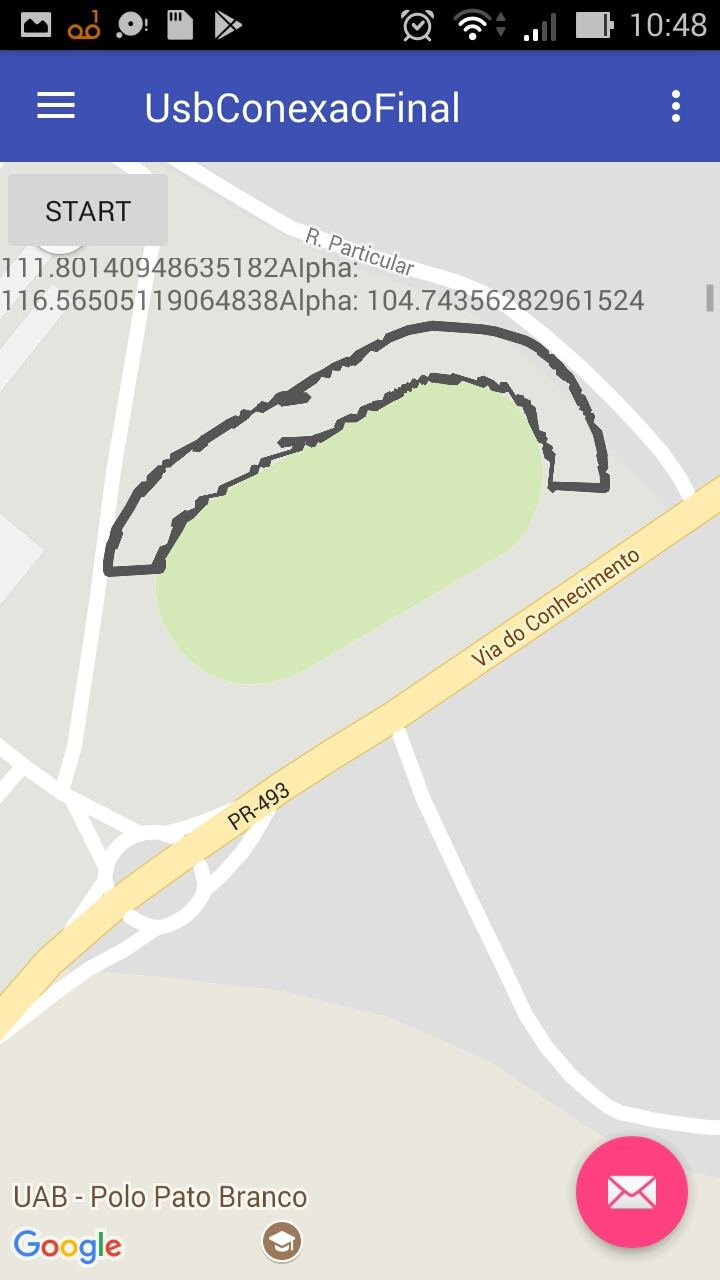
\includegraphics[width=0.5\textwidth,height=0.75\textheight,keepaspectratio]{Figuras/integracao.jpg}
	 \caption{Integração dos trabalhos desenvolvidos na Terris (Hamilton, Vinícius e Willian)}
	\end{figure}
	
\end{frame}




%%%%%%%%%%%%%%%%%%%%%%%%%%%%%%%%%%%%%%%%%%%%%%%%%%%%%%%%%%%%%%%%
\subsection{Implementação no microcontrolador}

\begin{frame}
\frametitle{Implementação no microcontrolador}
\begin{columns}

	\column{0.4\linewidth}
	\begin{itemize}
	\item Dados obtidos pela sentença GPRMC;
	\item Informações obtidas: longitude, latitude, velocidade de deslocamento e tempo de aquisição do sinal;
	\end{itemize}

	\column{0.7\linewidth}
	\begin{figure}[]
	 \centering
	 \captionsetup{width=0.9\textwidth,font=footnotesize,textfont=bf}
	 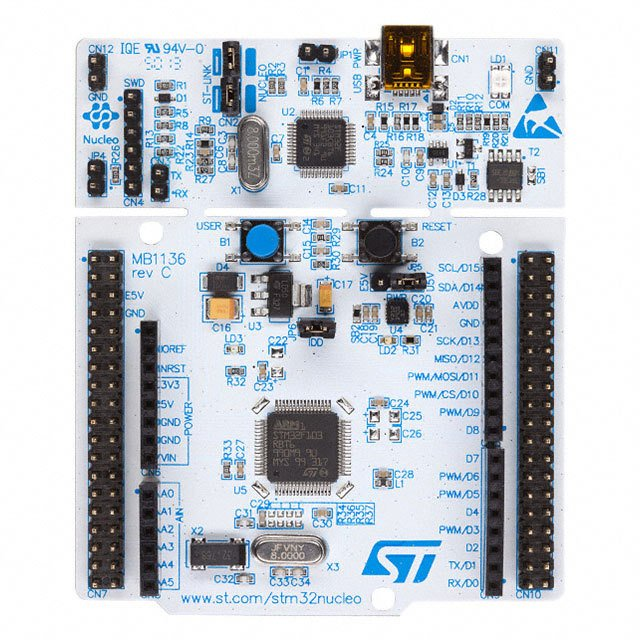
\includegraphics[width=0.9\textwidth,keepaspectratio]{Figuras/nucleo.jpg}
	 \vspace{-0.2cm}
	 \caption{Microcontrolador utilizado}
	\end{figure}
	
\end{columns}
\end{frame}

%%%%%%%%%%%%%%%%%%%%% EOF %%%%%%%%%%%%%%%%%%%%%%%